\documentclass[11pt]{article}
\usepackage[top=1.00in, bottom=1.0in, left=1.1in, right=1.1in]{geometry}
\usepackage{Sweave}
\renewcommand{\baselinestretch}{1.1}
\usepackage{graphicx}
\usepackage{natbib}
\usepackage{amsmath}
\usepackage{gensymb}
\usepackage{parskip}
\usepackage{xcolor}
\usepackage[disable]{todonotes}
\usepackage{xr-hyper}
\usepackage[utf8]{inputenc}
\externaldocument{workingdraftsupp}

\def\labelitemi{--}
\parindent=0pt

\begin{document}

\renewcommand{\refname}{\CHead{}}

% See also: git/grants/crc2023/crc2023app/docs/crc_notes2023more.tex which has some reference notes

\title{Climate change highlights fundamental gaps in\\ plant growth $\times$ growing season length relationships} % Do growing season length and growth relate? \\ And if not, why not? \\ And if we're not sure, why is that?
\author{Team Grephon}
\date{\today}
\maketitle



\begin{abstract}
Recently a growing number of studies have challenged a fundamental assumption of most forecasts of future climate climate---that longer growing seasons lead to increased tree growth---which predict increased plant growth will partly offset carbon emissions. A suite of diverse hypotheses, from increased drought and high temperatures, to internal limits on plant growth each year, have generally failed to coalesce around a predictive model of why longer growing seasons do, or do not, increase tree growth. Here, using a systematic literature review spanning regional, continental and global scales, we show: (1) an almost even divide in how often increased growing seasons are linked to increase growth---with 57\% of all papers finding a positive relationship across XX species, and (2) a fundamental disconnect between relevant fields---especially dendrochronology and plant physiology, which currently lead most research. Major hypotheses are generally studied uniquely by one field alone with little interdisciplinary research, limiting any development---or testing---of a mechanistic framework for when longer seasons should lead to greater growth. Leveraging current research, combined with theory from life history and community ecology, we outline how progress towards a predictive framework is possible, but will require both new fundamental science, alongside new approaches within and across disciplines. Currently untapped data could begin to test this ... 
\end{abstract}
% Ruben: We present a path towards building a mechanistic framework to predict the effect of longer seasons on tree growth. We suggest that lack of cross-disciplinary collaborations,and inconsistent terminology and testing approaches, are likely to explain why tree growth-phenology mechanisms remain poorly understood or outright untested. We discuss how easily accessible or already available data, currently untapped, has the potential to advance our understanding in this critical issue, and in turn greatly improve vegetation models.
% OLD: Here we highlight how progress could come from rising to the interdisciplinary challenge of this topic. Working across dendrochronology, ecology, life history, and physiology, we present a mechanistic framework for predicting when longer seasons should lead to greater growth.  While persistent biases in which disciplines study which mechanisms means much of the framework remains untested, we show that critical data---currently untapped---could rapidly advance our understanding, and in turn greatly improve vegetation models. % and highlight how poorly tested most mechanisms are.

\section*{Introduction}

The idea that longer growing seasons lead to increased plant growth is an intuitive tenet across multiple fields of biology, including physiology\todo{addcites}, dendrochronology\todo{addcites} and ecology. It is also a foundational assumption of most models of the future global carbon cycle\todo{addcites}. Most models project that future anthropogenic warming will be partly offset by increased carbon sequestration---primarily of temperate and boreal forests---as warming lengthens growing season\todo{addcites}, an assumption supported by a suite of ecosystem-scale studies \citep{finzi2020,keenan2014net}. Yet recent work has called this assumption into question.

A suite of recent studies have suggested longer growing seasons do not lead to greater tree growth \citep{dow2022warm,green2022limits,silvestro2023longer}, with potentially large implications for future climate change. This research suggests that limitations on plant growth mean forests will be limited sinks with increased warming. Such findings challenge decades of research that find growth does increase with longer seasons, from large-scale studies along natural elevational gradients\todo{addcites} to small-scale studies of cell growth in lab settings\todo{addcites} to previous studies of ecosystem fluxes with warming \citep{finzi2020,keenan2014net}. Proposed mechanisms for the apparent disconnect are highly diverse, from previously unknown fundamental internal limits on plant growth \citep{zohner2023effect} to effects of climate change itself, such as increased drought or temperatures too high for plant growth \citep{dow2022warm}, as well as differences simply due to the metric of growth \citep{green2022limits}.
% Studies that Green \& Keenan say no relationship:
	% Fatichi et al. 2014 (opinion)
	% Fatichi et al. 2019 (review)
	% JIang et al 2020 (FACE or sinilar) 

Here we review the connections between growing season length and plant growth across fields to identify the potential mechanisms that unite---and could disconnect---these processes. Our approach spans multiple fields to unify foundational studies with recent research related to anthropogenic warming. Leveraging a systematic literature review, we examine in which methods, species and approaches extended seasons appear to lead to increased growth, and the current proposed hypotheses. We find a pervasive disciplinary split between studies, which---we argue---limits our ability to identify the underlying processes. Further, we highlight critical insights from physiology, community ecology, and life history theory that have been unexamined in recent work. Taken together, the current fields studying connections between growing season length and growth appear primed to develop a holistic theory of when, where and how climate change may increase tree growth, with implications for both forecasts of future climate change and for fundamental science.
 
\section*{Evidence that longer seasons increase plant growth, or not}
%  (spanning 37 papers and 60 unique tests or studies; see Supp or Fig/Table)
The idea that time limits growth is a fundamental tenet across most biological fields. From the cellular to ecosystem levels, many biological processes are rate-limited in ways that tie back to time. Thus, the hypothesis that longer growing seasons should increase growth is intuitive---and pervasive. We found this was by far the most common hypothesis for why longer seasons should increase growth, across our systematic review of growth $\times$ growing season length studies, with 19 of XX total studies including it (see Supp). Foundational evidence for this relationship for plant growth come primarily from spatial clines across elevation and latitude, with growth decreasing alongside growing season length at higher elevations and latitudes (see Fig. XX). Mechanistically, this is supported by warming experiments that find species that advance phenologically with warming also perform better \citep[with performance most often measured by growth,][]{Cleland:2012}. With climate change, ecosystem-scale studies have reported a similar relationship across decades \citep{keenan2014net}. This, however, has not been well supported by recent work that has focused often on inter-annual correlations at the population- or individual-levels \citep{dow2022warm,silvestro2023longer}. This has led to debate about whether future carbon forecasts are overestimated and which metrics of growth \citep{green2022limits}, or growing season length \cite{korner2023four} are relevant.

Despite the recent eruption of this debate, we found little support for reports of a disconnect between growth and growing season length. Instead the field has generally found split support---across methods---for the when longer seasons lead to increased growth  Papers spanning XX to XX years have variously found evidence for---or not---the relationship, with no clear trend by method (Fig. XX). Thus, the path to understanding these results is unlikely to emerge solely through improved metrics. 

Studies from the disciplines of dendrochronology (tree-ring studies) and physiology have readily offered mechanisms for the recent results that increased growth may not come with longer seasons. External climatic drivers that offset the positive growth effects of longer seasons are often reported in tree ring studies\todo{addcites}, suggested when higher temperatures and lower precipitation produce negative correlations with growth\todo{addcites}. In contrast, several other studies suggested fundamental developmental constraints that prevent trees from responding to longer seasons\todo{addcites}. 

Yet we found that these hypotheses have been tested in radically different ways, never together, and ignore a suite of research on this topic---including other major possible mechanisms. Tree-ring studies have focused on external climatic drivers limiting growth in annual tree ring studies, while lab experimental and woody phenology (xylogenesis studies) focus on physiological constraints. Further, the consistency of varying results, with no clear pattern by method or even within species, suggests that understanding the relationship mechanistically will be critical to accurate predictions. As we outline below, a single mechanism is unlikely to explain all results, requiring more a more unified framework---and tests of it---for progress. 
 
\section*{Controllers on growth $\times$ growing season length relationships}

Here we examine the mechanisms that may limit or disrupt longer growing seasons leading to increased growth, integrating across the fields of dendrochronology, physiology, and ecology. A suite of mechanisms, both external---including climatic and biotic drivers---and internal can alter any simple growth x season length relationships. But a tendency to focus on only one or the other means we have little understanding of how they compare, or which may explain current findings. 

\subsection*{External}

\paragraph{Temperature \& moisture} % Abiotic

Fundamentally temperature limits biological processes. Temperatures that are too cool (often considered to be below 5\degree C for temperate trees) and too warm \citep[an area of active research][, see also Fig. \ref{fig:temperaturecomplex}]{martinez2008hot,cabon2022cross} slow down biological processes and eventually can lead to tissue death\todo{addcites}. Between the upper and lower limit biological processes underpinning growth generally accelerate such that warming can have a direct effect, effectively by accelerating biological time, up until the maximum rate for that particular process (Fig. \ref{fig:concepbiotime}).

Anthropogenic warming will thus shift a number of biological processes at the same time that it accelerates spring phenology, but will depend on the particular temperature response curve and exactly where along that curve warming will push the process. At very cool temperatures, a small increase in warming may have limited effect, whereas warming that pushes plant beyond their optima, where many rates crash, could have large impacts. In between, warming would linearly increase rates. Plant growth is likely then to shift with extended growing seasons at the same time it shifts due to changing rates, with some papers suggesting longer seasons effectively only extend the very cool periods and so have no discernable effect on growth (CITES), while others suggest observed increases in growth are due only to increased growth rates (not longer seasons) and finally a number tree ring studies seem to suggest and offset of growth due to high summer temperatures (CITES), though what temperatures are too high is not generally known, and it seems likely current temperatures are below the optima (CITES). 

Positive effects of longer seasons on growth are could also be offset by moisture deficits. If warming reduces soil moisture through either reduced precipitation or higher evaporation it could slow growth dramatically. A suite of tree ring studies confirm this, finding correlations with precipitation\todo{addcites} or other metrics related to plant access to water\todo{addcites}. The actual relationship between temperature, moisture and tree growth is more complex, as studies finding strong correlations between vapor pressure deficit and growth attest\todo{addcites}. 
% Temperature response curves assume sufficient moisture, with growth rapidly slowly ....

\paragraph{Species interactions} % Biotic

External factors related to species interactions---including herbivory, disease and competition---can also limit growth, and may themselves be responsive to an increasing growing season length. Herbivory can have large impacts on forests, leading to declines in satellite measures of greenness often associated of signals of plant senescence\todo{addcites}. And disease is well known to determine forest dynamics. Interestingly, these external factors have rarely been mentioned in studies examining growing season length (we found no mention of them in our literature review). 

\subsubsection*{Internal}

\paragraph{Universal limits} 
Plants internal programming could limit growth responses to longer seasons, with some constraints operating universally across species. These constraints can be genetic or developmental and include fundamental limits on plant processes through biophysical realities \citep[e.g., allometry, chemical reaction limits, and genetic architecture that may limit what trait combinations are possible][]{ackerly2000evolution}. Recent studies on how earlier seasons affect tree growth has focused strongly on developmental constraints, suggesting a never-before-heard-of role for the summer solstice to limit how much and when plants can invest in growth \citep{zohner2023effect}. This is hypothesized to be universal, somewhat contradicting decades of work showing species-level differences in how and when species grow. % This is hypothesized to be universal, somewhat contradicting decades of work showing local adaptation by populations, and species-level differences in `determinism' in growth x growing season length relationships. 

\paragraph{Species-specific limits}
Much internal programming that would affect growth responses varies by species, as evolution generally drives selection for different constraints and different strategies. Leaf strategies clearly vary strongly between evergreen and deciduous species, but also within each group---where variation in `determinism' defines a suite of choices on levels and timing of investment and leaf growth. Determinate species build most of their leaf material the season before and flush most leaf buds all at once at the start of season, while indeterminate species more continually produce new buds and flush them. Ideas of determinism, often used in forest sciences, intersect with ecological theories of different plant strategies along which species---especially within communities---assemble. Leaf, wood, fruit and other plant traits show trade-offs along a acquisitive to conservative axis: where some species can grow rapidly and more flexibly take advantage of resources, but are less defended against herbivores and compete poorly at low resource levels, whereas other species compete well at low resource levels, but at the expense of growing slower and conservatively \citep[][]{Grime:1977sw,diaz2016}. These ideas would predict indeterminate acquisitive species, such as poplar, to be far more likely to grow more with longer seasons, while conservative species, such as beech, may not. % Also say ring vs diffuse porous?
% Such strategies may also make predictions for reproductive investment, which---along with species-level differences---is almost wholly ignored in the current debate on the relationship between growth and growing season length.

Imprints of past selection, however, also drive species-level differences, producing phylogenetic patterns that may limit how well species are adapted to current conditions, and constrain plant responses \todo{addcites}. The legacy of historical evolutionary pressures---including different external drivers---is not easily erased.  Thus, many species show evidence of previous selection, seen when evolutionary relationships (usually represented through phylogeny) predict plant responses and lead to clade-level similarities. Most studies testing for such historical effects on plant responses find them, and even more physiological syntheses find results suggestive of strong phylogenetic relationships \citep[though they do not always test them, e.g.,][]{way2010differential}. 

\paragraph{Population- \& individual-level limits}
Below the species-level, variations from between-populations to within-individuals drive variation in growth and its relationship to growing season length. Populations often vary predictably in their end-of-season phenology, with more poleward populations tending to stop height growth (budset) earlier using locally adapted photoperiod cues \todo{addcites}. This means longer seasons---as defined by budset---are generally driven by spring phenology, which appears far more flexible, and has advanced more rapidly than fall events. Within populations, individual trees may also vary in how early or late they are for both spring and fall events. Within individuals maturity and shifting investment can drive inter-annual variation. Saplings tend to both grow more rapidly and have longer seasons relative to themselves as adult trees. Adult trees then vary depending on investment, most notably in reproduction. 

Trade-offs between vegetative and reproductive investments are a paradigm of life history theory and produce important differences across years within individuals (as well as between species). Years of high reproductive output can reduce growth (CITES). For species that mast---producing abundant cones or fruits in only some years---high reproduction years could especially impact measures of wood growth. Many hypotheses suggest higher summer temperatures trigger masting in the following year \citep{hacket2016tree,hacket2016consistent}; if true, then reduced growth in years following warm summers may not indicate temperatures too high for growth, as often suggested \citep[e.g.,][]{gantois2022new,dow2022warm}, but instead shifting investment in reproduction.



\section*{A cross-disciplinary framework for when longer seasons increase tree growth}
 
 % Building a mechanistic framework of when and where... 
 % These levels of complexity across diverse external and internal drivers make a suite of testable predictions.
Predicting when and where longer seasons lead to increased growth may seem overwhelming given the diversity of potential drivers, but together they offer a set of testable hypotheses that could rapidly advance progress---if tackled with a more organized and cross-disciplinary approach. Our literature review highlighted how siloed research is in the drivers they consider (see Fig. XX), with entire suites of hypotheses missing from the literature. 

Beyond failing to test a suite of highly relevant mechanisms, the lack of cross-disciplinary study means we lack coherent tests that compare multiple mechanisms. Dendrochronology considers almost exclusively external drivers, while physiological tests of constraints do not usually predict for which species, when and where constraints will be most important. Taken together, the current landscape of research suggests we may be testing a hypothesis for shifts with climate change that we never previously understood well in fundamental biology. 

Below we outline a path towards building a mechanistic framework to predict when the longer growing seasons of anthropogenic climate change will increase plant growth. This path requires building fundamental biological knowledge in a suite of areas across physiology, life history, tree rings, ecology and evolutionary biology. These suggestions thus apply to understanding this relationship at the individual (organismal level), though we highlight where they may make predictions are larger (e.g., ecosystem scales). % These suggestions apply to those wanting to specifically address hypotheses about the relationship between growing season length, phenology and growth at the individual (organism) level

\subsubsection*{Standardized measurements} % Box?

While our lit review showed that this doesn't matter, we also struggled to make an quantitative estimates -- so it does matter!

1.	What we measure should be standardized and common measurements (allow for communication across fields) for anyone who is interested in measuring growth and phenology at the individual level. This seems related having standard hypotheses and the graphs (Fredi and Ailene and Kavya<U+2019>s table, Cat<U+2019>s heat maps?). Specifically - 
a.	Standardize measurements of response variables when working on this question (growth, growing season length) AND explanatory variables (climate). We could provide table of standard measurements / units / approaches (assuming we can agree on this). Seems related to Ailene<U+2019>s document, and we can also cite Christian Korners paper<U+2026>
b.	Specific fields measuring relevant (individual) level metrics (growth, phenology) should ideally consider broadening what they measure (if easy) and / or addressing their biases. This will help future scientists conduct meta analyses. For example:
i.	If tree rings studies expanded to more measurements of angiosperms, this would allow for greater synthesis with phenology databases like PEP.
ii.	If phenological studies could focus more on both the start and end of the season (specifically, leafout and leaf fall), and make sure to focus on conifers / woody species, there would be more overlap with ITRDB.
iii.	For long-term forest growth plots, ensuring annual growth measurements paired with phenological measurements would help (most permanent plot data I know of, e.g. FIA and PSP, is collected every 5 years, no phenology). 
c.	We should also agree on a standardized set of analytical tools. E.g. tree ring analyses <U+2013> average away a lot of the interesting things. I<U+2019>m sure there are issues with phenological data, not sure what they are. 


\paragraph{Extending disciplinary focus}

\paragraph{Lags \& allocation}

\paragraph{Quantify species/population/individual variation}


\subsubsection*{Bridging the internal-external drivers divide}

\section*{Where to go in the batmobile now!}


Only a handful of studies mentioned species differences, and rarely made predictions based on existing theory. Shifting investment in growth versus reproduction, differences in plant strategies and phylogeny all predict testable variation in how growing season length impacts growth, but have been almost wholly ignored in the current debate. We argue this is because of a lack of cross-disciplinary study. For example, while evolutionary history, ecology and life history theory all predict differences across species, the two major disciplines currently studying this---physiology and dendrochronology---generally study either one species\todo{addcites}, lump all species in a site\todo{addcites}, or divide by one trait \citep[e.g.,][]{dow2022warm}. Research on trends over elevation, which seem foundational to understanding the growth x growing season length relationship, have been on a very limited species list---with almost no comparison across species. % Evolutionary history, ecology and life history theory all predict differences across species, but current analyses generally study either one species\todo{addcites}, or lump all species in a site\todo{addcites}.  

% Climatic drivers can clearly affect plant growth, but because they are generally tested by a field developed to derive climate signals from tree rings (dendrochronology), they are usually studied in isolation, with no way to compare their effects to biotic drivers, or internal constraints. 



But really predicting when the longer growing seasons of anthropogenic climate change will lead to increased growth requires building fundamental biological knowledge in a suite of areas across physiology, life history, tree rings, ecology and evolutionary biology. Careful cross-disciplinary is critical, but will benefit from shifts within disciplines. 








Both these [BIOTIC] drivers though can be more episodic and harder to measure, making them more difficult to easily test as mechanisms for limiting growth. In contrast, proxies for competition (such as surrounding tree density and identity), can be more easily measured, but are rarely studied. Mechanistic physiology studies rarely measure (or even include) competition and, given dendrochronology's focus on climatic signal through growth, the field similarly tries to avoid the study or impact of plant competition, even though it is foundational to forest dynamics. And ...  the very established method of merging into average site chronology reduces the chance of seeing competition or biotic factors in play.

 
 
%%%%%%%%%%%%%%%%%%%%%%%%%%%%%%%
%% OLD text -- minus stuff I cut and used already (I think) %%
%%%%%%%%%%% %%%%%%%%%%%%%%%%%%%%

% Text that I cut from the previous draft but may want to REVIEW to see if it's worth fitting in somewhere

Internal/External drivers



 ...though how much longer seasons are depends on what events define the start and end (CITES). 

Perhaps most remarkably unmentioned in the current debate is the prevalence of species-level differences ....

Beyond genetic and developmental constraints, evolutionary history can constrain plant responses\todo{addcites}, though this is effectively unstudied currently as a controller of how growing season length may be limited in affecting growth. Yet most studies testing for such historical effects on plant responses find them... though this is effectively unstudied currently as a controller of how growing season length may be limited in affecting growth. Further, many physiological syntheses find results suggestive of strong phylogenetic relationships, but fail to discuss or test them \citep[e.g., discussions of evergreen versus deciduous phenology without testing for whether this is actually correlated with the deep in time split between gymnosperms and angiosperms,][]{way2010differential}. '

% Previous draft text ... 

\emph{How warmer temperatures increase tree growth, or not}



Dendrochronology---the study of tree rings and their dating---has long assumed growth decreases with shorter seasons \citep[e.g.,][]{bruening2017}, though this connection is almost always made across space, not time. Elevation and latitude---two major factors that generally shorten seasons, and change a suite of climatic factors---generally lead to less annual growth (new Fig?). Most current work in dendrochronology assumes this relationship and focuses more on how climatic factors shift across these gradients\todo{addcites}. 

This focus on climatic signals in tree growth (measured by ring width) is the hallmark of dendrochronology, with the methods in the field generally designed around this aim. Statistical approaches attempt to remove periods of rapid growth with age. Sampling methods, at both the species and individual tree level, aim for the most climatic response (either to temperature or precipitation). This has led to a strong focus on conifers (gymnosperms), creating a major split from most studies of leaf phenology, which focus almost entirely on deciduous species (mainly angiosperms).
% Elevation and latitude---two major factors that generally shorten seasons, and change a suite of climatic factors---generally lead to less annual growth (new Fig?) though this relationship in reality may be more messy than many conceptual diagrams suggest. 



\emph{A cross-disciplinary framework for when longer seasons increase tree growth}


\emph{i. External drivers}

\emph{ii. Internal programming}







\emph{To the bat-mobile Robin! How to tackle this cross-disciplinary framework}





(\colorbox{cyan}{Hoping Janneke or someone wants to jump in somewhere here ...} in this section with our opinions on what people should measure, and something about statistical approaches?)


All fields would benefit from a deeper understanding of the physiological connections between growing season length and growth. Much work has focused on measures of growth and phenology without a clear mechanistic link. Similarly, many current suggestions of constraints lack any physiological mechanism. Physiological studies that follow carbohydrate and cell division versus expansion dynamics could yield insights. This is particularly important if want to include constraints in our projections, as extrapolating is especially dangerous when the underlying mechanistic model is wrong

Bridging across disciplines will require bridging across time-scales, a consistent and thorny issue for research into trees. We found most physiological studies of growth x growing season length relationships studied 1-2 years of dynamics, usually of juvenile trees, while tree ring studies are focused on synthesizing across decades or longer of adult tree growth. Perhaps because of this dichotomy, tree ring studies often study lag effects\todo{addcites}, while they are rarely mentioned in physiological studies. Given the complexity of carbon storage in trees \citep{finzi2020,thompson2023no,anderson2022drives}, and how investment can shift across years\todo{addcites}, we argue more studies should acknowledge and test for lag effects. Integrating more research from ecology and field global change experiments could help. Large scale experiments on heat (e.g., SPRUCE), moisture via drought or irrigation (e.g., DroughtNet, Phynwald) and other factors (e.g., $CO_2$ in FACE) have increasingly been used to test ecological `memory' and could help scale up from smaller and shorter-time scale physiological studies.

Dendrochronology provides an invaluable long-term perspective, but using it to understand tree growth beyond climatic factors will require new perspectives and approaches. As rings are easiest to observe in conifers, and conifers often exist in the most extreme climatic places (and thus have more clear signal of climate on growth), dendrochronology has limited data for species where phenology may be most strongly tied to growth---deciduous species, which are mostly angiosperms. Phenology and dendrochronology are somewhat unique fields in biology for their open data that is both geographically and temporally deep; yet the overlap in comparable data due to each field focusing mostly on different suites of species is incredibly limited (\colorbox{orange}{New fig here of PEP725 x ITRB data?}). Further, most standard statistical methods for `standardizing' tree ring data are focused on enhancing climatic signals---which could schmear insights into growing season length or other factors, especially for studies across populations \citep{de2022temperature}. The fundamental model of growth in dendrochronology could use revisiting, especially as new mechanistic understanding from physiology advances. Layering on the complexity of growth depending not only temperature and precipitation, but on vapor pressure deficit, as well as losses in growth that are more episodic (e.g., frost, disease) would help.

From these shifts in physiological and tree ring studies, could come more comparable quantitative estimates---which we currently lack. While multiple papers report a lack of relationship between growth and growing season length, we have no fundamental understanding of what the effect size of this relationship should be, and thus no way to know if we have good power in current studies to detect it. Estimates of how growth shifts with elevation likely include responses from both plasticity and local adaptation and thus could be an upper bound on our expectations, yet elevational trends to date appear relatively weak and noisy (Fig. \ref{fig:gxelev})---suggesting a suite of missing mechanistic understanding. Additionally, observational studies must attempt to tease out effects of high temperatures that should accelerate the rate of plant growth, from longer seasons, and from temperatures that are too high and stall growth. Without a solid basis for the underlying temperature response curve, such attempts are likely non-identifiable statistically, and thus could easily report underlying correlations between predictors as signals of different temperature and season-length responses [\colorbox{orange}{More on VPD and/or xylogenesis here?}]. And these complexities must be addressed through a multi-species lens.

While tackling these challenges for multiple species alone can seem daunting, allowing for and studying differences between species may remove much of the noise in current studies. Species-level variation in growth is a repeated prediction and finding of both life history theory and community ecology, and both yield expectations of which species should differ the most. Species with acquisitive versus conservative traits, and which differ in their reproductive strategies (i.e., masting or not, fruit size and number) should form the basis of choosing which species to focus on for further study and to test predictions. Acquisitive species with consistent investment in fruit would show stronger shifts in growth with changing growing season length---assuming no other factors become limiting. Given the potential role of evolutionary history, selecting for these varying strategies within a clade, or---if not feasible---correcting for phylogenetic distance would more robustly test how strategies influence the growth x growing season length relationship. Studies across more species, or careful synthesis of studies across species, could test for the role of evolutionary history.

Getting a handle on species-level variation is super-duper important as we need to understand the scale of it versus other levels of variation, and compared to other drivers of variation. Current studies of how growing season length influences growth have worked at a variety of scales, with many recent ones focusing on inter-annual variation within individuals (or ecosystems) while previous work across space more likely compared populations, with almost none comparing species. Partitioning this variation requires studies that sample carefully at each level, then statistically separate out variation. 

Theory clearly predicts species are unlikely to share a common growth x growing season length relationship, but less research addresses how the relationship should shift across populations. \emph{In situ} elevation work suggests no genetic differences \citep{king2013tree}, while common garden studies across latitudes suggest phenological variation across populations limits growth \citep{soolanayakanahally2013timing}, though most work is not comparable as common garden studies rarely report annual ring width. Given that many common garden studies have some data on phenology\todo{addcites} and are designed to tease out population versus inter-annual variation, collecting tree ring data from them seems a rapid way to estimate variation across these two levels, and could be combined with species level variation. Given how old some common gardens are, research may also be able to examine impacts of biotic and abiotic disturbances or effects of climatic variation.

Disentangling the effects of major drivers on growth---from growing season length, to temperature, moisture and constraints---likely requires experiments. To date, few experiments have teased out the effects of warmer temperatures versus an longer season, and none---to our knowledge---have carefully measured growth. Such experiments, however, will be critical in establishing a baseline understanding of the role of season length alone in determining growth. And they can compare species robustly. Advancing them to extend the season via early growth or delayed senescence, and layering on heat waves or drought treatments could provide comparable estimates and test lag effects (when sampled multiple years after the manipulations). While these are most easily done for juvenile trees, they could be done on adult trees (given the infrastructure investment), giving the opportunity to measure impacts on reproductive output as well. 
% Comparing the effects of various drivers on growth---from growing season length, to temperature, moisture and constraints---may be impossible from observational or experimental approaches alone. Each is limited ... 

\emph{Conclusions:}
Anthropogenic climate change has often been described as an unfortunate, unnatural, and unreplicated experiment. What this often hints at is how much it has highlighted important biology we don't know well, and how much it requires us to rediscover dusty old fundamentals, while also exposing their limits---and thus our limits of understanding. When, how and why longer seasons lead to increased tree growth will require a multi-discplinary reckoning with how temperature, growth and biological time affect plant growth. But we need to figure it out, because getting this right is important for our future forest dynamics, and the suite of species and services that depend on them. And that includes carbon sequestration---which, we really need now! 


\emph{Misc text without a home...}

Disciplinary work could also rapidly advance our understanding, especially if designed to be comparable across disciplines. Tree ring studies are inherently focused on growth through ring width, but reporting frost events, biotic disturbances, reproduction status of trees and considering mast years would acknowledge additional mechanisms. Physiological studies tend to avoid such complexities through controlled environments and a focus on juvenile plant stages, but scaling up between life stages is critical. Bridging this gap would be aided by physiological studies reporting metrics similar to ring width, alongside their more common measurements of shoot elongation, height and biomass. 

This framework predicts longer growing seasons will increase growth for species with regular reproduction (no masting), an acquisitive strategy, from clades that are historically (on an evolutionary timescale) plastic, in locations that are warm---but not too warm---and moist. Further earlier growth should not drive increased frost damage, herbivory, or disease... Go test it, preferably in some mid-latitude, temperate forest for a species not too close to the edge of its range.


i. Hypotheses for why GSL x growth is not found are not equally tested across fields: Constraint issues in provenance but not tree ring etc.\\
ii. Our premise is that some hypotheses for what is going may be tractably already answered by combining data across fields/methods\\
iii. And, you could go far by cross-field tweaking of what each field is doing

\iffalse
Most global models of future warming assume increased anthropogenic carbon will be offset by increased carbon sequestration in forests as growing seasons lengthen.

The proposed mechanisms for this, however, are highly diverse---and most studies measure different aspects of growth across widely varying spatial and temporal scales. 

A positive link between longer growing seasons and increased carbon sequestration 

A suite of recent studies have called into question this fundamental assumption .... failed to find a link between longer seasons and increased tree growth

This assumption appeared well supported by several large-scale studies of ecosystem fluxes 
\fi


\newpage
\section{Box. ``Growth", measured how, exactly?}
Tree growth can be measured in a variety of ways. Our systematic review found most studies quantified growth by measuring radial growth (e.g., through increment cores or dendrometers, $n=$28), but a number also looked at metrics related to C assimilation (e.g. net ecosystem productivity or gross primary productivity, $n=$20), while a smaller number examined biomass, height, or number of stems ($n=$9), or root:shoot ratio ($n=$1). Some studies used modeled estimates of photosynthesis \citep[e.g.,][relies on daily photosynthesis estimates derived from the LPJ-GUESS photosynthesis model, Smith et al 2014]{zohner2023effect},\citep[][estimates photosynthese using the Integrated Terrestria Ecosystem C-budget model(InTEC), Chen et al 2000]{chen2000}. Others measured photosynthesis at the leaf level, through flux towers, or used greenness metrics (NDVI). 

Growth measurements vary across disciplines and study types, posing a further challenge to an interdisciplinary approach to understanding how growing season length relates to growth. Greenhouse or growth chamber studies and provenance trials are more likely to measure height or biomass, whereas larger scale syntheses and remote-sensed studies are more likely to use metrics of carbon assimilation. 

Aligning across the range of growth metrics will be critical for an integrated understanding of growth-growing season length relationships and implications under continued climate change.  There is decoupling among some metrics of growth. For example, vegetation photosynthesis may be poorly correlated with tree radially growth, and this relationship can vary seasonally \citep{cabon2022cross}. Further, tree radial growth is not a perfect indicator of whole tree growth, since plants allocate
carbon to their roots, leaves, reproductive structures, and stores in addition to wo aboveground biomass. Relationships among different metrics of growth are not simplistic, so selecting relevant ones and aligning across the most widely used ones will be necessary, though not easy: the relationship  between photosynthesis, radial growth, and carbon uptake has large implications for future carbon sequestration and it remains widely debated \citep{green2022limits}.


\newpage
\section{Figures}
\begin{figure}[h!]
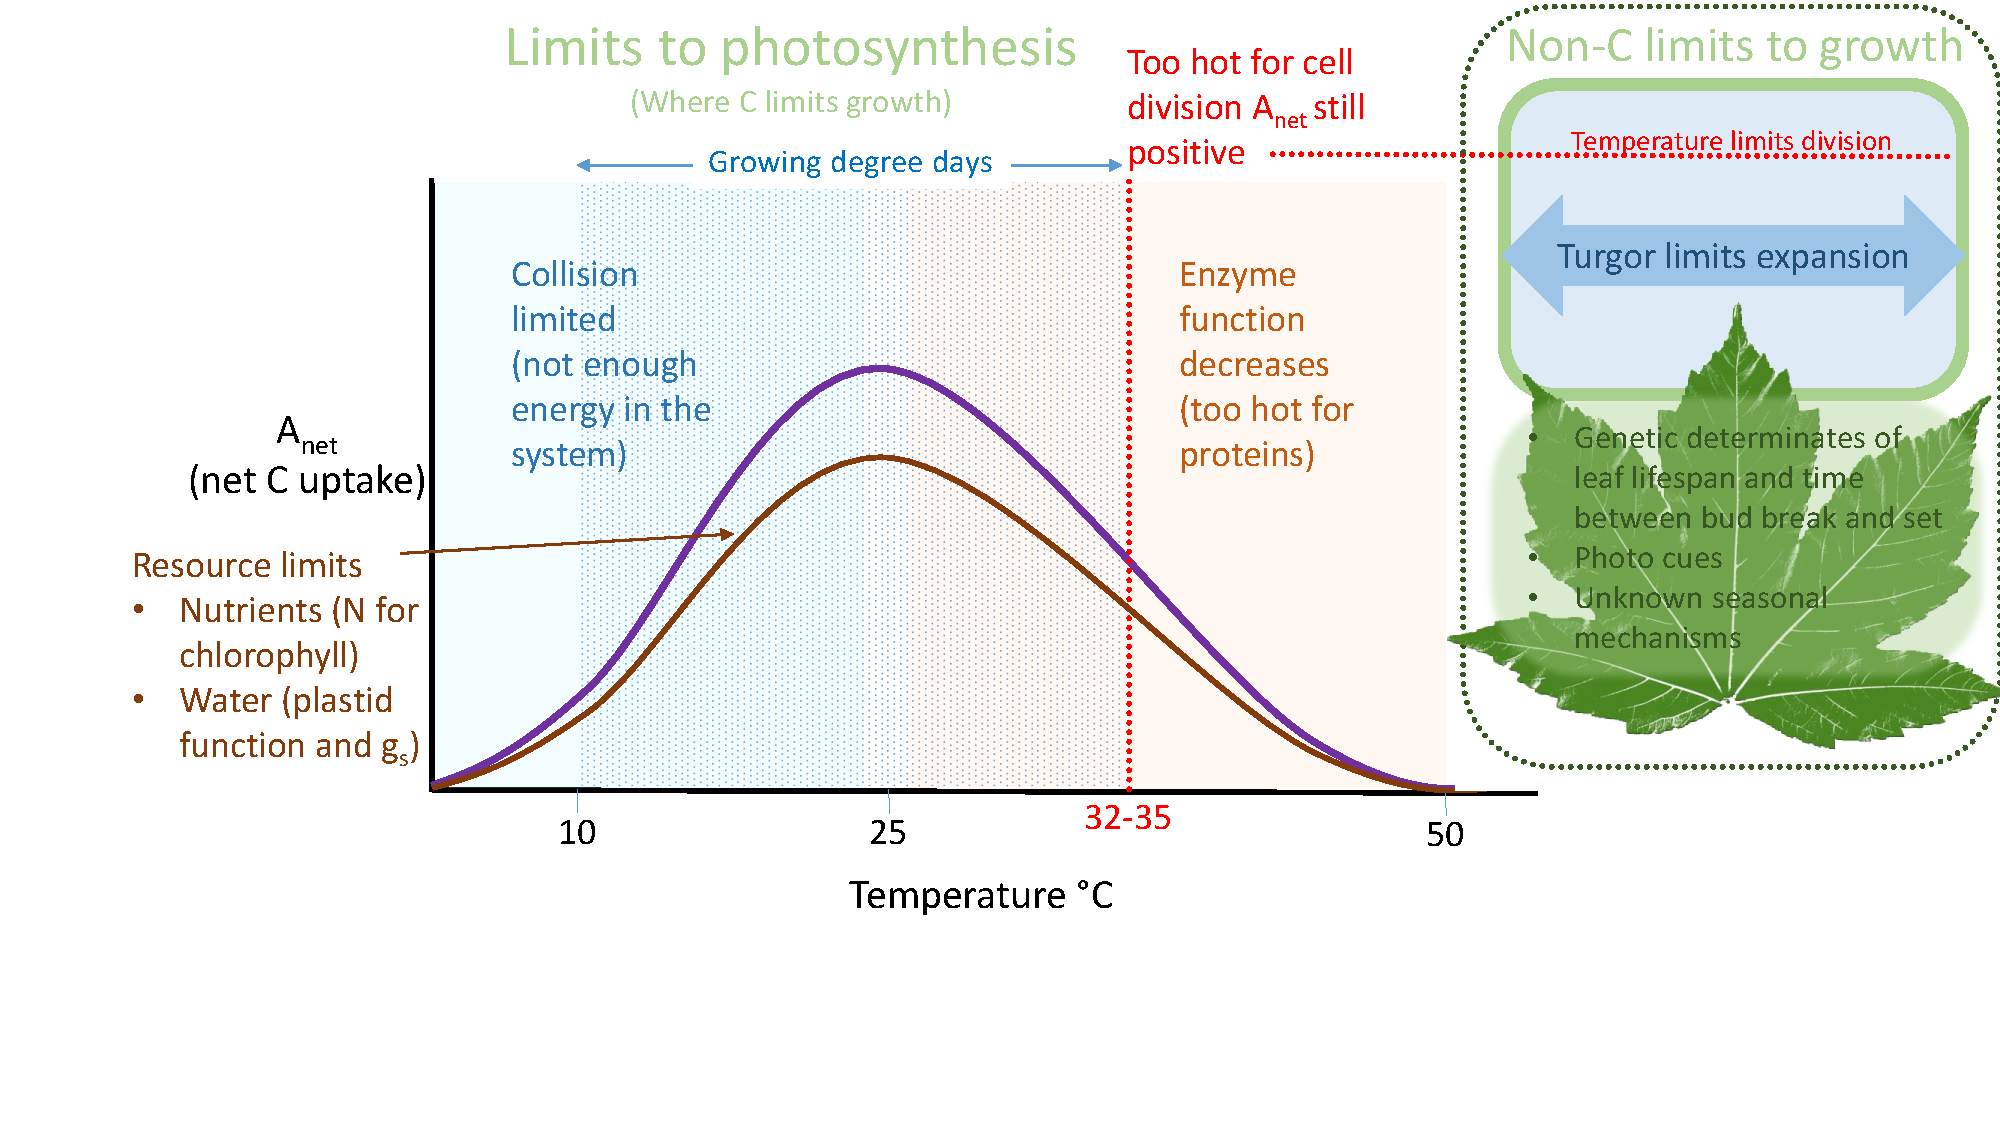
\includegraphics[width=1\textwidth]{..//figures/grephonfig.pdf}
\caption{Less simplified version of how temperature works, including lots of limits at high and low temperatures.}
\label{fig:temperaturecomplex}
\end{figure}


\begin{figure}[h!]
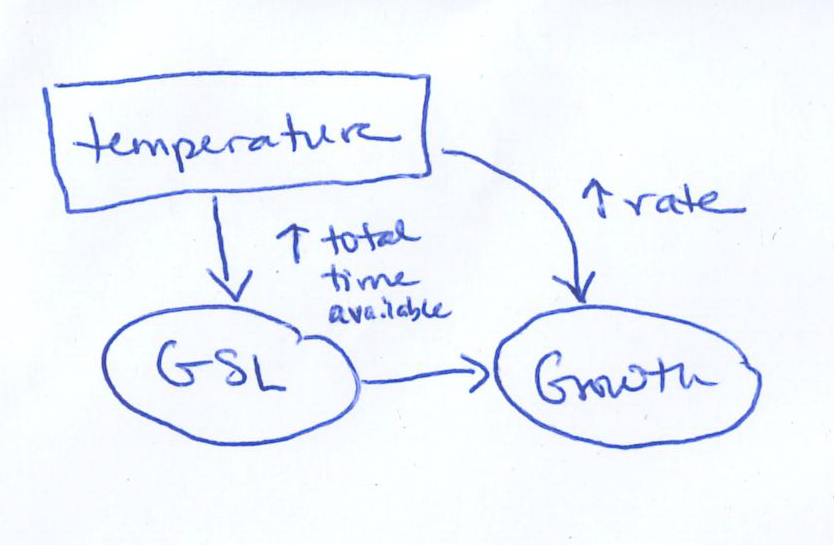
\includegraphics[width=0.5\textwidth]{..//figures/gsltogrowth/gsltogrowth_emw1a.png}
\caption{Idealized simplified version of the world, where resources (including water, N etc.) are abundant and temperatures are never too cool or too hot. In this world, temperature can increase growth directly (through increasing the speed of biological processes, up to some limit) and indirectly, but increasing the absolute available time for those processes to happen and lead to more growth.}
\label{fig:concepbiotime}
\end{figure}


\begin{figure}[h!]
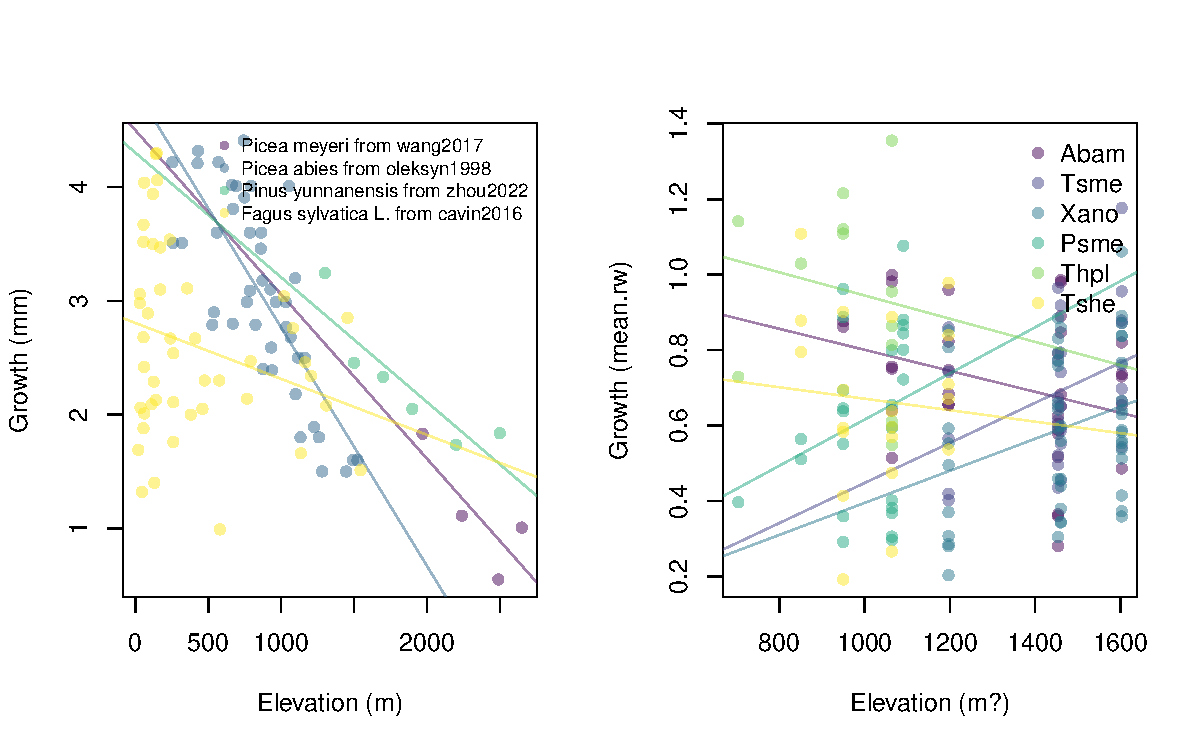
\includegraphics[width=1\textwidth]{..//analyses/growthxelevationetc/figures/growthxelev2part.pdf}
\caption{Literature review of growth x elevation studies (left) and results from Mount Tahoma/Rainier (right).}
\label{fig:gxelev}
\end{figure}


\begin{figure}[h!]
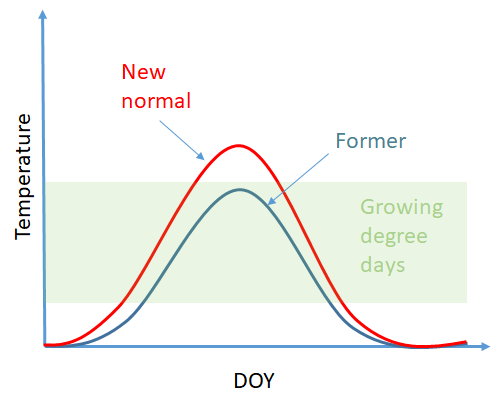
\includegraphics[width=0.75\textwidth]{..//figures/simpletempcurve_fromlucidboard.png}
\caption{Simplified version of how GDD works before and after climate change.}
\label{fig:simpletemp}
\end{figure}




\begin{figure}[h!]
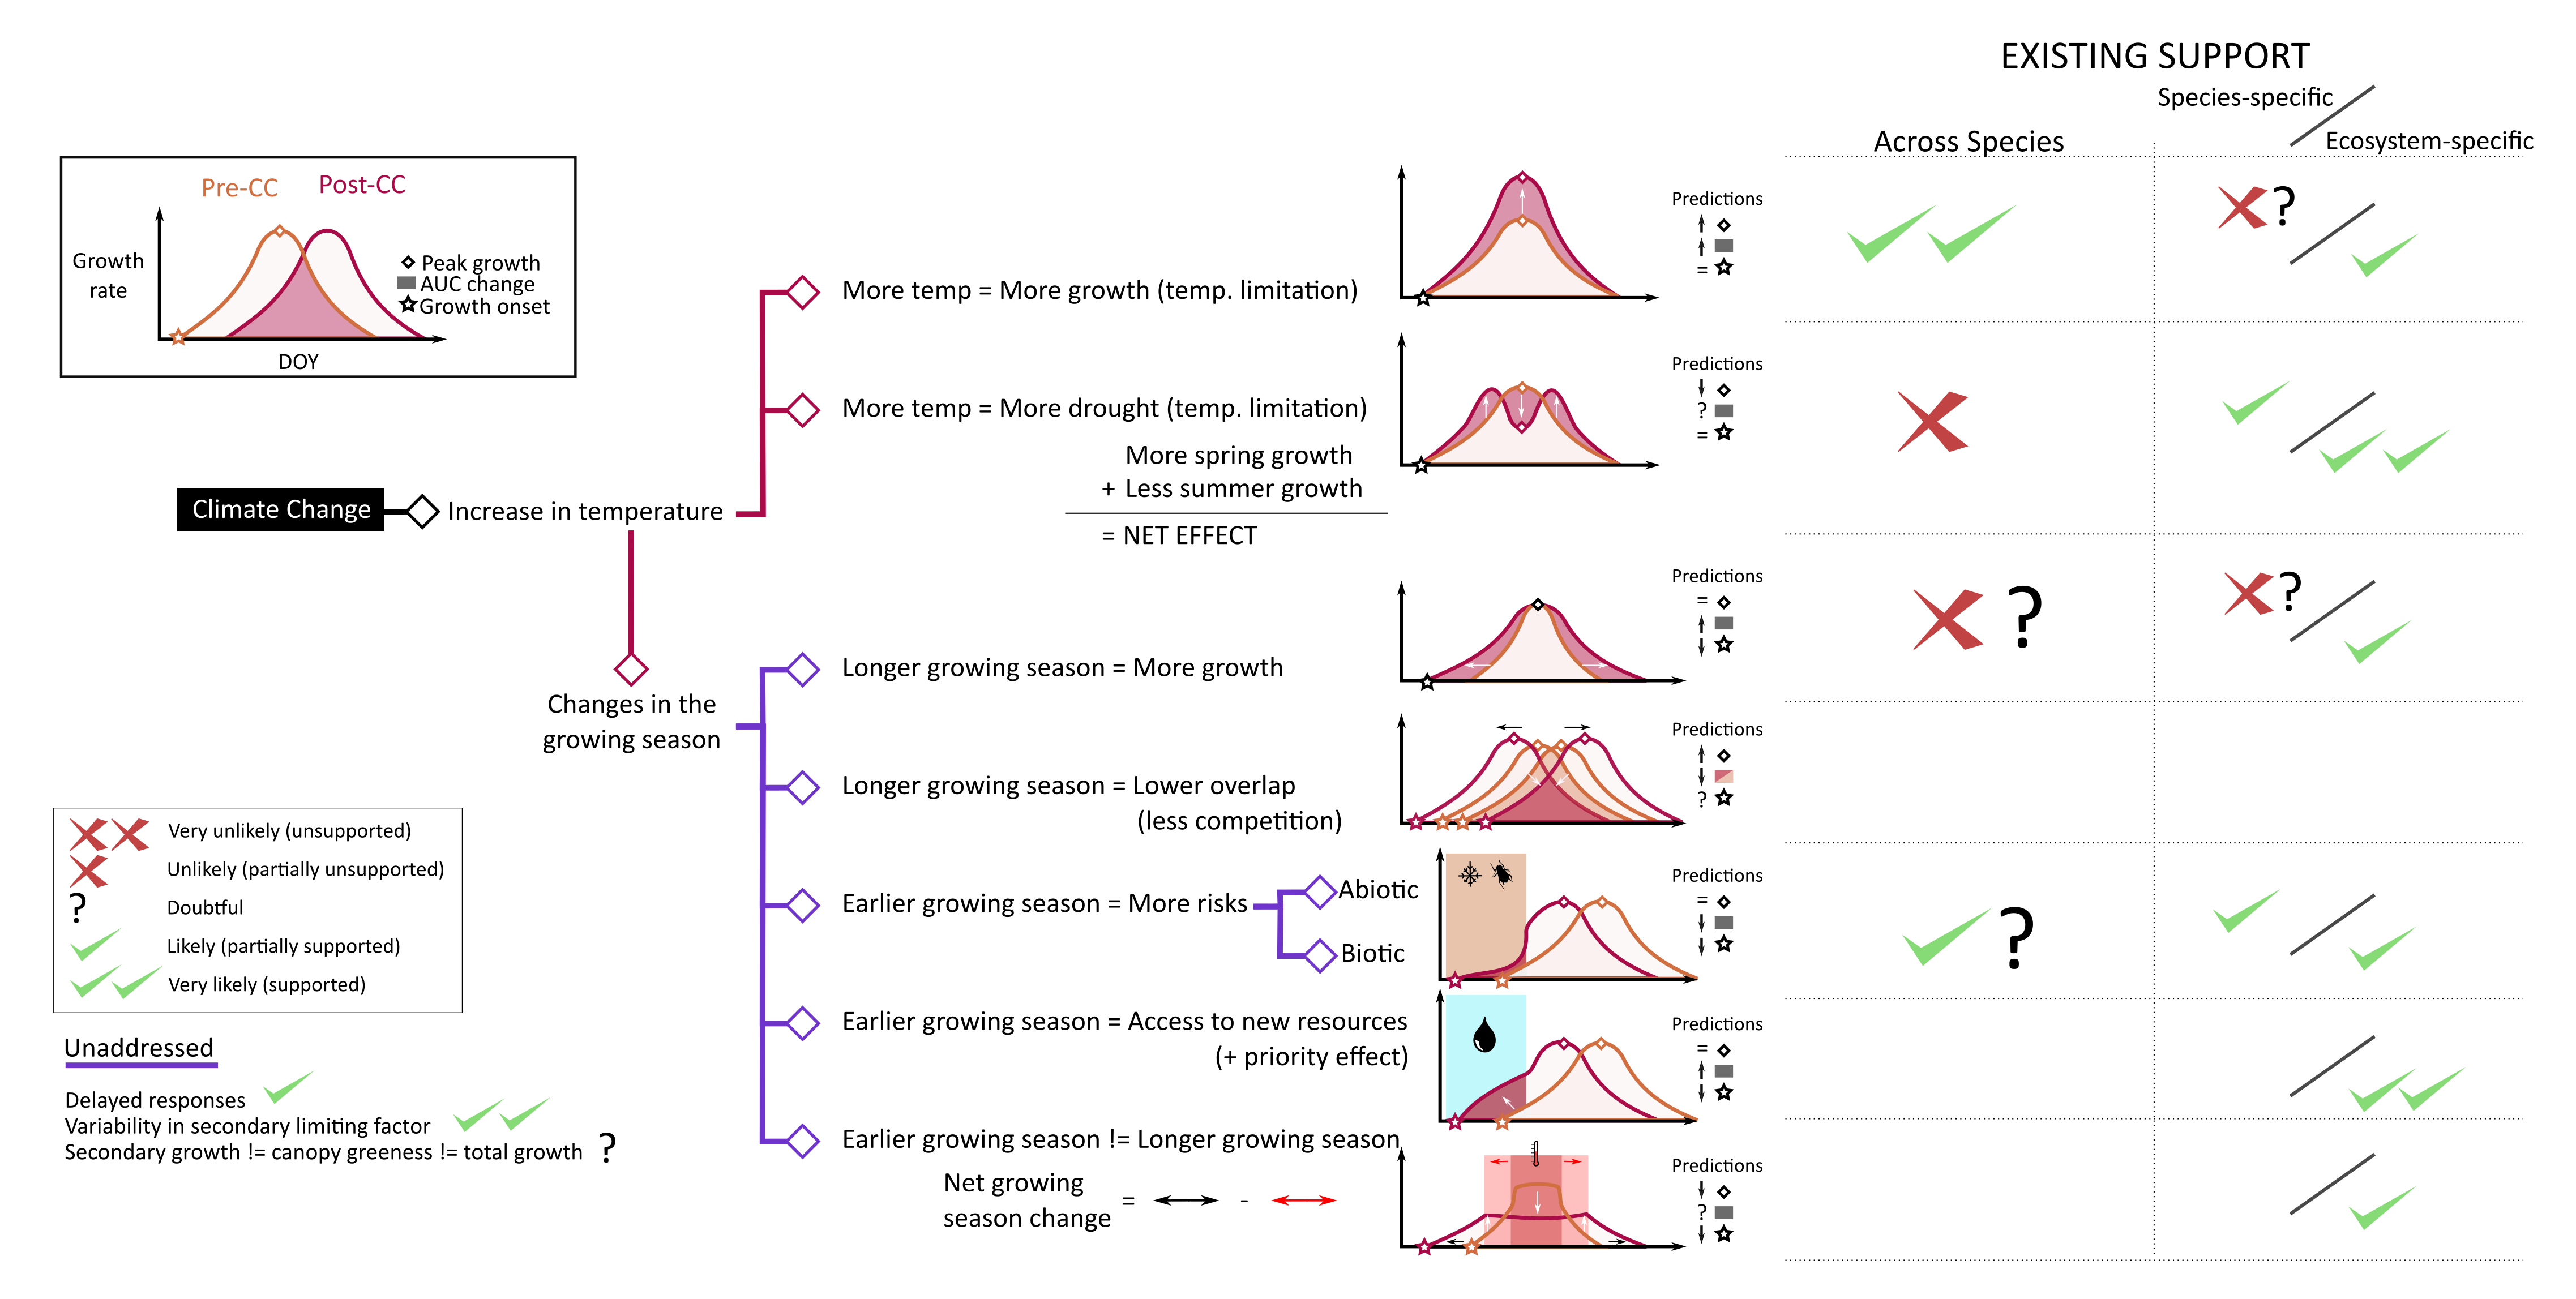
\includegraphics[width=1\textwidth]{..//figures/some conceptual figure2.0.png}
\caption{Pathways through which climate change could alter growing season length and growth.}
\label{fig:pathways}
\end{figure}


\clearpage
\section{References}
\bibliography{..//bibtex/grephonbib}
\bibliographystyle{/Users/Lizzie/Documents/git/bibtex/styles/besjournals.bst}

\clearpage

\section{Old take home results from table}

\emph{{\bf Warnings \& disclaimers:}
I flip between counting papers at the start to looking more at rows, so you were forewarned on that. }




\section{Getting back to writing our paper}

\emph{Reminder of what we expected the table we worked on since April to help us with ...}
\begin{enumerate}
\item Section: Review three reasons for not growing 
\begin{enumerate} 
\item Overview paragraph of three reasons
\begin{enumerate} 
\item Measurement -- see box/figure  (include measurement only here or briefly so we move through it fast)
\item Resource limitation
\item Constraints
\end{enumerate}
\item Resource limitation, evidence for an against \todo{Table will help us with this}
\begin{enumerate}
\item Nutrients
\item Water
\item Is this more species-specific?
\end{enumerate}
\item Constraints, evidence for an against \todo{Table will help us with this}
\begin{enumerate}
\item Leaf life span
\item Budset stuff ... (Zohner, Sool.)
\item Evidence across species? Or which is species-specific
\end{enumerate}
\end{enumerate}
\item What do do next (The future! Is there a framework to our future directions? It would be nice if we found one) \todo{This needs a total overhaul after the table; figure out the section headers}
\end{enumerate}





\end{document}


